%% Copyright 1998 Pepe Kubon
%%
%% `two.tex' --- 2nd chapter for thes-full.tex, thes-short-tex from
%%               the `csthesis' bundle
%%
%% You are allowed to distribute this file together with all files
%% mentioned in READ.ME.
%%
%% You are not allowed to modify its contents.
%%

%%%%%%%%%%%%%%%%%%%%%%%%%%%%%%%%%%%%%%%%%%%%%%%%%
%
%     Chapter 5   
%
%%%%%%%%%%%%%%%%%%%%%%%%%%%%%%%%%%%%%%%%%%%%%%%%

\chapter{A MinHash-based Method}
\label{ch:hashing}

In this chapter, we use the MinHash~\cite{Broder97} technique, a locality-sensitive hashing (LSH) scheme, to approximate Jaccard similarity. We design indices for efficient updating estimated similarity scores. Since the MinHash technique is designed for estimating sets rather than multi-sets, we slightly change the definition of the current query to the set of distinct elements in the current sliding window. 
% In Section~\ref{sec:static-minHash}, we . Our methods for is presented in Section~\ref{sec:evolve-minHash}. 

\section{Top-$k$ Similarity Search for Static Queries}\label{sec:static-minHash}

We first discuss how to estimate Jaccard similarity using MinHash for static objects and queries. 

% Let $h(A)$ denote a list of hash values for all the elements in set $A$ and $\min (h(A))$ be the minimum value in $h(A)$. We can use the following property to approximate Jaccard similarity scores. 

% redefine, add how hash functions are generated

\begin{definition}[Image under Permutation~\cite{URL:imagePerm}]\label{def:permutation}
Let $[n]$ denote the set $\{0,\dots,n-1\}$. A permutation $\pi$ on $[n]$ is a bijective function (one-to-one correspondence) from $[n]$ to itself. If $x \in [n]$, then $\pi(x)$, the value of $\pi$ when applied to $x$, is the image of $x$ under $\pi$. The image of a subset $X \subseteq [n]$ under $\pi$ is defined as follows.

$$\pi[X] = \{y\,|\,y=\pi(x) \text{ for each } x \in X\}$$

%The two-row notation of $\pi$ is written as two rows of elements in $[n]$ as the following.

%\[ 
%\pi = 
%	\begin{bmatrix}
%	0 & 1 & \cdots & n-1 \\ 
%	\pi(0) & \pi(1) & \cdots & \pi(n-1)
%	\end{bmatrix}
%\]

\end{definition}


\begin{definition}[Min-Wise Independent Permutations~\cite{Broder98min-wiseindependent}]\label{def:minwise}
Let $S_n$ be the set of all permutations of $[n]$. A family of permutations $\mathcal{F} \subseteq S_n$ is min-wise independent if for any set $X \subseteq [n]$ and any element $x \in X$, we have
$$Pr(\min\{\pi[X]\} = \pi(x)) = \frac{1}{|X|}$$
where the permutation $\pi$ is chosen randomly in $F$, $\pi[X]$ is the image of $X$ under $\pi$, and $\pi(x)$ is the image of $x$ under $\pi$.
\end{definition}

% add definition of the minwise independent hash function
\begin{property}[Jaccard Similarity Estimation~\cite{P01}]
\label{pminh}
Let us consider a query $q$ and an arbitrary object $T_i$ in which the elements are drawn from a lexicon, $\Sigma$. Let $h$ be a hash function that maps elements in $\Sigma$ to distinct integers in range $[0, |\Sigma|-1]$ and is randomly picked from a family of min-wise independent permutations as discussed in Definition~\ref{def:minwise}. Also, let the MinHash value, $\min(h(T_i))$, be the element in $T_i$ with the smallest hash value. Jaccard similarity between $T_i$ and $q$ can be estimated using the following equation.           
$$Pr[\min(h(T_i))=\min(h(q))]=\frac{|T_i \cap q|}{|T_i \cup q|}$$ 
\end{property}


%\begin{table}[tb] 
%\caption{Signature Matrix} 
%\label{sigMatrix}
%\centering
%    \begin{tabular}{|c||c|c|c|c|c|c|c|c|c|c|} \hline 
%      &$q$&$T_1$&$T_2$&$T_3$&$\cdots$&$T_{m-1}$&$T_m$\\ \hline \hline
%      $h_1$&&&&&&&\\ \hline
%      $h_2$&&&&&&&\\ \hline
%      $h_3$&&&&&&&\\ \hline
%      $\vdots$&&&&&&&\\ \hline
%      $h_{l-1}$&&&&&&&\\ \hline
%      $h_l$&&&&&&&\\ \hline
%    \end{tabular} 
%\end{table}

The MinHash values for all objects and that of the query can be stored in a MinHash signature matrix, $M$, where each entry $M(i, j)$ is the MinHash value of the $j^{th}$ itemset under hash function $h_i$. Based on Property~\ref{pminh}, the Jaccard similarity between two itemsets can be estimated by the ratio of the number of rows containing the same MinHash values to the number of all the rows in the signature matrix. The detailed computation is shown in Example~\ref{examinh}.



%\begin{table}[tb]
%\centering
%\caption{Comparison on Exact and Estimated Jaccard Similarity}
%\setlength{\tabcolsep}{2\tabcolsep}
%\setlength{\tabcolsep}{0.8\tabcolsep}\resizebox{70mm}{!}
%{
%     \begin{tabular}{|c||c|c|c|c|c|c|} \hline 
%      $sim_{Jac}(T_i, q)$&$T_1$&$T_2$&$T_3$&$T_4$\\ \hline 
%      Estimated&0.40&0.20&0.60&0.40\\ \hline
%      Exact&0.40&0.25&0.75&0.40\\ \hline
%    \end{tabular} }
%\setlength{\tabcolsep}{0.5\tabcolsep}
%\label{estScores}
%\end{table}

\begin{table*}[tb]
\centering
\caption{An Example of Jaccard Similarity Estimation}
\label{JacSimEstExa}
\subfigure[Matrix Representation of Sets]{% g
\centering
%\centering\resizebox{40mm}{!}
{
    \begin{tabular}{|c||c|c|c|c|c|} \hline 
      Element & $T_1$ &$T_2$&$T_3$&$T_4$&$q$\\ \hline 
      $a$&1&1&0&1&0\\ \hline
      $b$&1&0&1&0&1\\ \hline
      $c$&1&0&1&0&1\\ \hline
      $d$&0&1&0&1&1\\ \hline
      $e$&0&0&1&1&1\\ \hline
    \end{tabular}}
\label{MatrixEx}}
\quad 
\subfigure[Random Permutations]{% h
\centering
% \centering \resizebox{55mm}{!}
{
     \begin{tabular}{|c||c|c|c|c|c|} \hline 
      Element & $h_1$ &$h_2$&$h_3$&$h_4$&$h_5$\\ \hline 
      $a$&1&2&3&1&0\\ \hline
      $b$&2&3&0&3&4\\ \hline
      $c$&3&0&1&4&3\\ \hline
      $d$&4&4&2&0&1\\ \hline
      $e$&0&1&4&2&2\\ \hline
    \end{tabular}}
\label{HashFunc}}
\quad
\subfigure[Signature Matrix for Example~\ref{examinh}]{% h
\centering
\setlength{\tabcolsep}{2\tabcolsep}
%\resizebox{60mm}{!}
{
     \begin{tabular}{|c||c|c|c|c|c|} \hline 
      &$T_1$ &$T_2$&$T_3$&$T_4$&$q$\\ \hline \hline
      $h_1$&$a$&$a$&$e$&$e$&$e$\\ \hline
      $h_2$&$c$&$a$&$c$&$e$&$c$\\ \hline
      $h_3$&$b$&$d$&$b$&$d$&$b$\\ \hline
      $h_4$&$a$&$d$&$e$&$d$&$d$\\ \hline
      $h_5$&$a$&$a$&$e$&$a$&$d$\\ \hline
    \end{tabular}}
\setlength{\tabcolsep}{0.5\tabcolsep}
\label{sigMEx1}}
\quad
\subfigure[Comparison on Exact and Estimated Jaccard Similarity]{% h
\centering
\setlength{\tabcolsep}{2\tabcolsep}
{
     \begin{tabular}{|c||c|c|c|c|c|c|} \hline 
      $sim_{Jac}(T_i, q)$&$T_1$&$T_2$&$T_3$&$T_4$\\ \hline 
      Estimated&0.40&0.20&0.60&0.40\\ \hline
      Exact&0.40&0.25&0.75&0.40\\ \hline
    \end{tabular} }
\setlength{\tabcolsep}{0.5\tabcolsep}
\label{estScores}}
\end{table*}

\begin{example} [Jaccard Similarity Estimation] \label{examinh} 
% add detailed explanation of each table.
% add top-k, compare to exact
We consider the matrix representation of four objects and a static query $q$ shown in Table~\ref{MatrixEx}. Each column in the matrix represents a set and an element is in the set if the corresponding entry is $1$. We apply five random permutations defined in Table~\ref{HashFunc}, as the min-wise independent hash functions, on objects and the query and get the signature matrix shown in Table~\ref{sigMEx1}. For example, since object $T_1$ contains element $a$, $b$, and $c$, the corresponding hash values according to $h_4$ are $1$, $3$, and $4$, respectively. The MinHash value of $T_1$ according to $h_4$ is $a$ since $a$ is the element in $T_1$ with the smallest hash value.   

Then, we can estimate the Jaccard similarity score between two sets by computing the ratio of the number of rows containing the same MinHash values to the number of random permutations. For example, the MinHash values of $T_1$ and $q$ are the same according to random permutations $h_2$ and $h_3$. Thus, the estimated Jaccard similarity between $T_1$ and $q$ is $\frac{2}{5}$. We compare the estimated Jaccard similarity with the exact Jaccard similarity for each object in Table~\ref{estScores}. When objects are ordered in descending estimated similarity score regarding the query, we have $T_3 > T_1 = T_4 > T_2$, which is identical to the order using exact similarity. Therefore, in this example, we can get the top-$k$ result accurately using estimated scores.         
\end{example} 


\section{Top-$k$ Similarity Search over Evolving Queries}\label{sec:evolve-minHash}
\begin{table}[tb]
\centering
\caption{Notations used by MinHash-based Algorithms}
% \small
\begin{tabular}{|l| p{10cm}  |} \hline
      Notation & Interpretation \\ \hline
      $mh(q_t)$ & A list of MinHash values of $q_t$ according to $l$ hash functions. \\ \hline
      $mh_i(q_t)$ & The MinHash value of $q_t$ according to the $i^{th}$ hash function, $h_i$, $i \in [1, l]$. \\ \hline
      $S_{T_j}$ & The estimated similarity score between $T_j$ and the current query, $j \in [1, m]$.\\ \hline
      $I_i$ & Inverted index built on the MinHash values of the $i^{th}$ hash function, $i \in [1, l]$.\\ \hline
      $I_i(v)$ &  Inverted list of hash value $v$ which consists of the objects whose MinHash value is $v$ according to the $i^{th}$ hash function, $i \in [1, l]$ and $v \in [1,|\Sigma|]$. \\ \hline
\end{tabular}
  \label{Notations}
\end{table}  

To answer evolving queries, given a fixed set of hash functions, the MinHash values for all the objects are fixed and only the MinHash values for the query are subject to modification. That is, we only need to update the MinHash values for the query. Therefore, we have a straightforward solution shown in Algorithm~\ref{minHashBasic}. Table~\ref{Notations} lists the symbols used in the MinHash-based algorithms for ease of presentation. Algorithm~\ref{minHashBasic} first computes the MinHash signature for the updated query. To determine if we shall update the estimated Jaccard similarity of object $T_j$ regarding the updated query $q_t$ according to a hash function $h_i$, we consider the following $4$ cases based on whether the MinHash values of the object and the queries are equal or not.

\begin{algorithm2e}[t]
 \SetAlgoLined%\small
 \SetKwInput{Input}{Input}
 \SetKwInput{Output}{Output}
 \caption{A MinHash-based Algorithm (MHB)} 
 \label{minHashBasic}
 \Input{$q_t$; $l$ hash functions; $mh(q_{t-1})$; MinHash table for $m$ objects.}
 \Output{$topk_{t}$}

 Compute $mh(q_{t})$\;
 \ForEach{$j \in \{1,...,m\}$}{
  \ForEach{$i \in \{1,...,l\}$}{
  \uIf{$mh_i(T_j) \neq mh_i(q_{t-1})$ and $mh_i(T_j) = mh_i(q_{t})$}
  {$S_{T_j} \gets S_{T_j}+\frac{1}{l}$\;}
    \uElseIf{$mh_i(T_j) = mh_i(q_{t-1})$ and $mh_i(T_j) \neq mh_i(q_{t})$}
  {$S_{T_j} \gets S_{T_j}-\frac{1}{l}$\;}
   }
  \If{$T_j$ $\not \in topk_t$ and $S_{T_j} > \min_{heap\_element}$}
  {Update $topk_t$\;}
   }
\end{algorithm2e}   


\begin{itemize}
\item Case 1: If $mh_i(T_j) \neq mh_i(q_{t-1})$ and $mh_i(T_j) = mh_i(q_{t})$, the estimated Jaccard similarity between $T_j$ and the updated query should be increased by $\frac{1}{l}$ where $l$ is the number of hash functions applied. 
\item Case 2: If $mh_i(T_j) = mh_i(q_{t-1})$ and $mh_i(T_j) \neq mh_i(q_{t})$, the estimated Jaccard similarity between $T_j$ and the updated query should be decreased by $\frac{1}{l}$. 
\item Case 3: If $mh_i(T_j) = mh_i(q_{t-1})$ and $mh_i(T_j) = mh_i(q_{t})$, we do not change the estimated Jaccard similarity between $T_j$ and the updated query.
\item Case 4: If $mh_i(T_j) \neq mh_i(q_{t-1})$ and $mh_i(T_j) \neq mh_i(q_{t})$, we do not change the estimated Jaccard similarity between $T_j$ and the updated query.
\end{itemize} 


Thus, for each hash function, the estimated Jaccard similarity of an object $T_j$ regarding the updated query changes only when Case $1$ and Case $2$ occur.
% when the MinHash value of $T_j$ equals to the MinHash value of $q_{t}$ but does not equal to the MinHash value of $q_{t-1}$, and vice versa. 
The time complexity of this algorithm is $O(l\cdot m)$, where $m$ is the number of objects and $l$ is the number of hash functions used for estimating the similarity scores.   




%\begin{example} [Updating Top-$k$ Result using MHB] \label{topkMHB} 
%\end{example} 

We can further reduce the computational cost using inverted indices. The MinHash signature matrix that stores the MinHash values of objects can be transformed into $l$ inverted indices whose structure is shown in Figure~\ref{InvIndices}. For each hash function, its corresponding inverted index stores a mapping from each existing MinHash value to a list of object ids, \emph{i.e.}, inverted list. Moreover, elements in each inverted list are sorted in ascending order of object id, which enable more efficient list merge and intersection operations. In this way, we can efficiently retrieve the objects with a specified MinHash value according to a certain hash function. 

\begin{figure}[t]
  \caption{Inverted Indices for MinHash Values}
  \label{InvIndices}
  \centering
    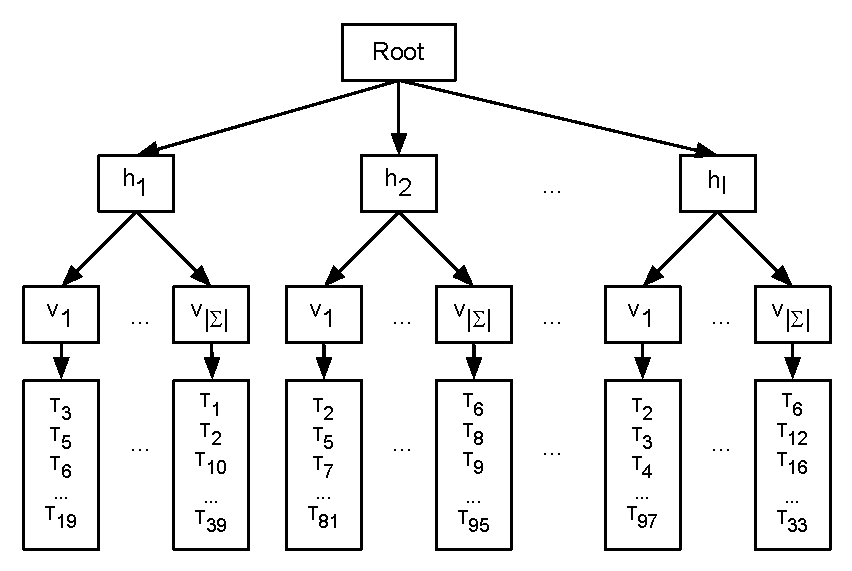
\includegraphics[width=0.7 \textwidth]{fig/invertedIdx.pdf}
\end{figure}


\begin{table*}[tb]
\centering
\caption{An Example of Inverted Indices for MinHash Values}
\label{invMinHash}
\subfigure[Index for $h_1$]{% g
%\centering
%\centering\resizebox{40mm}{!}
\setlength{\tabcolsep}{4\tabcolsep}
{
    \begin{tabular}{|l|} \hline
      $a: T_1, T_2$ \\ %\hline
      $e: T_3, T_4$  \\ \hline
\end{tabular}
}
\setlength{\tabcolsep}{0.25\tabcolsep}
\label{invh1}}
\quad 
\subfigure[Index for $h_3$]{% h
%\centering
% \centering \resizebox{55mm}{!}
\setlength{\tabcolsep}{4\tabcolsep}
{
     \begin{tabular}{|l|} \hline
      $b: T_1, T_3$ \\ %\hline
      $d: T_2, T_4$ \\ \hline
\end{tabular}}
\setlength{\tabcolsep}{0.25\tabcolsep}
\label{invh3}}
\quad 
\subfigure[Index for $h_5$]{% h
%\centering
% \centering \resizebox{55mm}{!}
\setlength{\tabcolsep}{4\tabcolsep}
{
     \begin{tabular}{|l|} \hline
      $a: T_1, T_2, T_4$ \\ %\hline
      $e: T_3$  \\ \hline
\end{tabular}}
\setlength{\tabcolsep}{0.25\tabcolsep}
\label{invh5}}
\quad 
\subfigure[Index for $h_2$]{% h
%\centering
% \centering \resizebox{55mm}{!}
\setlength{\tabcolsep}{4\tabcolsep}
{
     \begin{tabular}{|l|} \hline
      $a: T_2$ \\ %\hline
      $c: T_1, T_3$ \\ %\hline
      $e: T_4$  \\ \hline
\end{tabular}}
\setlength{\tabcolsep}{0.25\tabcolsep}
\label{invh2}}
\quad 
\subfigure[Index for $h_4$]{% h
%\centering
% \centering \resizebox{55mm}{!}
\setlength{\tabcolsep}{4\tabcolsep}
{
     \begin{tabular}{|l|} \hline
      $a: T_1$ \\ %\hline
      $d: T_2, T_4$ \\ %\hline
      $e: T_3$  \\ \hline
\end{tabular}}
\setlength{\tabcolsep}{0.25\tabcolsep}
\label{invh4}}
\end{table*}   



\begin{algorithm2e}[thb]
 \SetAlgoLined
 \SetKwInput{Input}{Input}
 \SetKwInput{Output}{Output}
 \caption{A MinHash-based Algorithm using Inverted Indices (MHI)} 
\label{minHashInd}
 \Input{$q_t$; $l$ hash functions; $mh(q_{t-1})$; inverted indices.}
 \Output{$topk_{t}$}
 Compute $mh(q_{t})$\;
  \ForEach{$i \in \{1,...,l\}$}{
 \If{$mh_i(q_{t-1}) \neq mh_i(q_{t})$}{
 \For{$T_j \in I_i(mh_i(q_{t}))$}{$S_{T_j} \gets S_{T_j}+\frac{1}{l}$\;}
 \For{$T_j \in I_i(mh_i(q_{t-1}))$}{$S_{T_j} \gets S_{T_j}-\frac{1}{l}$\;}
 }
 }
 Find $topk_{t}$ using updated scores\;
\end{algorithm2e}

\begin{example} [Inverted Indices for MinHash Values] \label{indexMinHash} 
Let us consider the objects in Example~\ref{examinh}. The inverted indices for all $5$ hash functions are shown in Table~\ref{invMinHash}.       
\end{example}


An algorithm that uses the inverted indices is presented in Algorithm~\ref{minHashInd}. The MinHash signature for the updated query is computed firstly. We need to search the inverted index of a hash function $h_i$ only when the MinHash values of $q_t$ and $q_{t-1}$ regarding $h_i$ are different. Suppose the MinHash value of the updated query has changed according to $h_i$, to determine which objects' similarity scores to update, we recall Case $1$ and Case $2$ mentioned earlier in this section. Each case corresponds to a scan in an inverted list of $h_i$. To be more precise, corresponding to Case $1$, we increase the estimated Jaccard similarity by $\frac{1}{l}$ for objects in the inverted list of hash value $mh_i(q_{t})$. That is, instead of checking for each object as in Algorithm~\ref{minHashBasic}, we search for the objects that satisfy Case $1$ utilizing the index. Similarly, we decrease the estimated Jaccard similarity by $\frac{1}{l}$ for objects in the inverted list of hash value $mh_i(q_{t-1})$, which corresponds to Case $2$. 

The worst case of this algorithm is $O(l\cdot m)$, where $m$ is the number of objects and $l$ is the number of hash functions. It is achieved when the MinHash values of consecutive queries differ under all the hash functions. However, this case could hardly occur because the Jaccard similarity between consecutive queries is in fact very high. On the other extreme, the best case of this algorithm is $O(l)$ when the MinHash signature of the current query is exactly the same as that of the previous query.  

% and is above $\frac{n-1}{n+1}$ where $n$ is the sliding window size. Thus, on average, the MinHash values would not change under $\frac{n-1}{n+1}\cdot l$ hash functions. We only need to explore $\frac{2}{n+1}\cdot l$ hash functions in each update.

\begin{table}[t]
\centering
\caption{Comparison on Exact and Estimated Jaccard Similarity for Example~\ref{topkMHI}}
\setlength{\tabcolsep}{2\tabcolsep}
% \setlength{\tabcolsep}{0.8\tabcolsep}\resizebox{70mm}{!}
{
     \begin{tabular}{|c||c|c|c|c|c|c|} \hline 
      $sim_{Jac}(T_i, q_t)$&$T_1$&$T_2$&$T_3$&$T_4$\\ \hline 
      Estimated&$0.80$&$0.20$&$0.60$&$0.40$\\ \hline
      Exact&$0.75$&$0.20$&$0.75$&$0.60$\\ \hline
    \end{tabular} }
\setlength{\tabcolsep}{0.5\tabcolsep}
\label{topkMHIcomp}
\end{table}

\begin{example} [Updating Top-$k$ Result using MHI] \label{topkMHI} 
Let us continue the example for estimating Jaccard similarity discussed in Example~\ref{examinh}. Suppose $k=1$, the top-$1$ object is $T_3$ regarding query $q_{t-1}=\{c, d, b, e\}$. At time $t$, the query is updated to $q_t=\{d, b, e, a\}$. The MinHash signature lists for $q_{t-1}$ and $q_t$ are $[e, c, b, d, d]$ and $[e, c, b, a, a]$, respectively. Based on Algorithm~\ref{minHashInd}, we only need to search the inverted index of $h_4$ and $h_5$ since the MinHash signatures of $q_{t-1}$ and $q_t$ only differ in $2$ positions.       
   
Using the inverted lists computed in Example~\ref{indexMinHash}, for $h_4$, we decrease the estimated similarity score by $0.20$ for objects in $I_4(d) = \{T_2, T_4\}$ and increase the estimated similarity score by $0.20$ for objects in $I_4(a) = \{T_1\}$. We follow the same procedure for $h_5$. The estimated Jaccard similarity regarding the updated query is shown in Table~\ref{topkMHIcomp}. The top-$1$ object suggested by Algorithm~\ref{minHashInd} becomes $T_1$.   
      
\end{example}





